\documentclass[12pt,twoside]{article}
%%%%%%%%%%%%%%%%%%%%%%%%%%%%%%%%%%%%%%%%%%%%%%%%%%%%%%%%%%%%%
% Meta informations:
\newcommand{\trauthor}{Ali Saleh}
\newcommand{\trtype}{Seminar Paper} %{Seminararbeit} %{Proseminararbeit}
\newcommand{\trcourse}{Bio-Inspired Artificial Intelligence}
\newcommand{\trtitle}{On the usage of Deep Learning Methods in Object Detection and Recognition}
\newcommand{\trmatrikelnummer}{6517831}
\newcommand{\tremail}{3saleh@informatik.uni-hamburg.de}
\newcommand{\trdate}{18.12.2013}
%%%%%%%%%%%%%%%%%%%%%%%%%%%%%%%%%%%%%%%%%%%%%%%%%%%%%%%%%%%%%
% Languages:

% Falls die Ausarbeitung in Deutsch erfolgt:
% \usepackage[german]{babel}
% \usepackage[T1]{fontenc}
% \usepackage[latin1]{inputenc}
% \usepackage[latin9]{inputenc}	 				
% \selectlanguage{german}

% If the thesis is written in English:
%\usepackage[english]{babel} 						
%\selectlanguage{english}

%%%%%%%%%%%%%%%%%%%%%%%%%%%%%%%%%%%%%%%%%%%%%%%%%%%%%%%%%%%%%
% Bind packages:
\usepackage{acronym}                    % Acronyms
\usepackage{algorithmic}								% Algorithms and Pseudocode
\usepackage{algorithm}									% Algorithms and Pseudocode
\usepackage{amsfonts}                   % AMS Math Packet (Fonts)
\usepackage{amsmath}                    % AMS Math Packet
\usepackage{amssymb}                    % Additional mathematical symbols
\usepackage{amsthm}
\usepackage{booktabs}                   % Nicer tables
%\usepackage[font=small,labelfont=bf]{caption} % Numbered captions for figures
\usepackage{color}                      % Enables defining of colors via \definecolor
\definecolor{uhhRed}{RGB}{254,0,0}		  % Official Uni Hamburg Red
\definecolor{uhhGrey}{RGB}{122,122,120} % Official Uni Hamburg Grey
\usepackage{fancybox}                   % Gleichungen einrahmen
\usepackage{fancyhdr}										% Packet for nicer headers
%\usepackage{fancyheadings}             % Nicer numbering of headlines

%\usepackage[outer=3.35cm]{geometry} 	  % Type area (size, margins...) !!!Release version
%\usepackage[outer=2.5cm]{geometry} 		% Type area (size, margins...) !!!Print version
%\usepackage{geometry} 									% Type area (size, margins...) !!!Proofread version
\usepackage[outer=3.15cm]{geometry} 	  % Type area (size, margins...) !!!Draft version
\geometry{a4paper,body={5.8in,9in}}

\usepackage{graphicx}                   % Inclusion of graphics
%\usepackage{latexsym}                  % Special symbols
\usepackage{longtable}									% Allow tables over several parges
\usepackage{listings}                   % Nicer source code listings
\usepackage{caption}
\usepackage{multicol}										% Content of a table over several columns
\usepackage{multirow}										% Content of a table over several rows
\usepackage{rotating}										% Alows to rotate text and objects
\usepackage[hang]{subfigure}            % Allows to use multiple (partial) figures in a fig
%\usepackage[font=footnotesize,labelfont=rm]{subfig}	% Pictures in a floating environment
\usepackage{tabularx}										% Tables with fixed width but variable rows
\usepackage{url,xspace,boxedminipage}   % Accurate display of URLs

%%%%%%%%%%%%%%%%%%%%%%%%%%%%%%%%%%%%%%%%%%%%%%%%%%%%%%%%%%%%%
% Configurationen:

\hyphenation{whe-ther} 									% Manually use: "\-" in a word: Staats\-ver\-trag

%\lstloadlanguages{C}                   % Set the default language for listings
\DeclareGraphicsExtensions{.pdf,.svg,.jpg,.png,.eps} % first try pdf, then eps, png and jpg
\graphicspath{{./src/}} 								% Path to a folder where all pictures are located
\pagestyle{fancy} 											% Use nicer header and footer

% Redefine the environments for floating objects:
\setcounter{topnumber}{3}
\setcounter{bottomnumber}{2}
\setcounter{totalnumber}{4}
\renewcommand{\topfraction}{0.9} 			  %Standard: 0.7
\renewcommand{\bottomfraction}{0.5}		  %Standard: 0.3
\renewcommand{\textfraction}{0.1}		  	%Standard: 0.2
\renewcommand{\floatpagefraction}{0.8} 	%Standard: 0.5

% Tables with a nicer padding:
\renewcommand{\arraystretch}{1.2}

%%%%%%%%%%%%%%%%%%%%%%%%%%%%
% Additional 'theorem' and 'definition' blocks:
\theoremstyle{plain}
\newtheorem{theorem}{Theorem}[section]
%\newtheorem{theorem}{Satz}[section]		% Wenn in Deutsch geschrieben wird.
\newtheorem{axiom}{Axiom}[section] 	
%\newtheorem{axiom}{Fakt}[chapter]			% Wenn in Deutsch geschrieben wird.
%Usage:%\begin{axiom}[optional description]%Main part%\end{fakt}

\theoremstyle{definition}
\newtheorem{definition}{Definition}[section]

%Additional types of axioms:
\newtheorem{lemma}[axiom]{Lemma}
\newtheorem{observation}[axiom]{Observation}

%Additional types of definitions:
\theoremstyle{remark}
%\newtheorem{remark}[definition]{Bemerkung} % Wenn in Deutsch geschrieben wird.
\newtheorem{remark}[definition]{Remark} 

%%%%%%%%%%%%%%%%%%%%%%%%%%%%
% Provides TODOs within the margin:
\newcommand{\TODO}[1]{\marginpar{\emph{\small{{\bf TODO: } #1}}}}

%%%%%%%%%%%%%%%%%%%%%%%%%%%%
% Abbreviations and mathematical symbols
\newcommand{\modd}{\text{ mod }}
\newcommand{\RS}{\mathbb{R}}
\newcommand{\NS}{\mathbb{N}}
\newcommand{\ZS}{\mathbb{Z}}
\newcommand{\dnormal}{\mathit{N}}
\newcommand{\duniform}{\mathit{U}}

\newcommand{\erdos}{Erd\H{o}s}
\newcommand{\renyi}{-R\'{e}nyi}
%%%%%%%%%%%%%%%%%%%%%%%%%%%%%%%%%%%%%%%%%%%%%%%%%%%%%%%%%%%%%
% Document:
\begin{document}
\renewcommand{\headheight}{14.5pt}

\fancyhead{}
\fancyhead[LE]{ \slshape \trauthor}
\fancyhead[LO]{}
\fancyhead[RE]{}
\fancyhead[RO]{ \slshape \trtitle}

%%%%%%%%%%%%%%%%%%%%%%%%%%%%
% Cover Header:
\begin{titlepage}
	\begin{flushleft}
		Universit\"at Hamburg\\
		Department Informatik\\
	\end{flushleft}
	\vspace{3.5cm}
	\begin{center}
		\huge \trtitle\\
	\end{center}
	\vspace{3.5cm}
	\begin{center}
		\normalsize\trtype\\
		[0.2cm]
		\Large\trcourse\\
		[1.5cm]
		\Large \trauthor\\
		[0.2cm]
		\normalsize Matr.Nr. \trmatrikelnummer\\
		[0.2cm]
		\normalsize\tremail\\
		[1.5cm]
		\Large \trdate
	\end{center}
	\vfill
\end{titlepage}


%%%%%%%%%%%%%%%%%%%%%%%%%%%%
% Abstract:

% Abstract gives a brief summary of the main points of a paper:
\section*{Abstract}
  Machine Learning algorithms depends highly on how you present the data to the algorithm and a successful algorithm can grasp info and details from the presented data, a multi-level learning algorithm use different layers of feature detectors so that each layer can grasp several aspects and features of the input data and be used as a new data input for the next layer this method can be viewed as searching the input space from several different views and leads to grasping more info about the input than that grasped by any other non-hierarchical algorithm. this paper will give an introduction about Deep learning , previous work, and current breakthroughs.It will also give a deeper explanation for a recent attempt to use a deep hierarchical algorithms to detect and recognize objects in images and how this algorithm can be scaled to be used with real time applications.

% Lists:
\setcounter{tocdepth}{2} 					% depth of the table of contents (for Seminars 2 is recommented)
\tableofcontents
\pagenumbering{arabic}
\clearpage

%%%%%%%%%%%%%%%%%%%%%%%%%%%%
% Content:

% the actual content, usually separated over a number of sections
% each section is assigned a label, in order to be able to put a
% crossreference to it

\section{Introduction}
\label{sec:introduction}
One of the earliest research fields that mathematicians and computer scientists have been working on is the idea of a machine that can show a presumably intelligent behavior. 
This led to many attempts to define intelligence and ways to measure it \cite{turing1950computing} and a sub-fields begun to shape many ways to simulate human intelligence using machines, and a usual way to tackle a AI problem is to decompose it to a number of sub-problems that solving each collectively simulate the original problem in a way that can be accepted as intelligence. Currently there are several ways to form a mathematical model that can learn and simulate human behavior,  while supervised models have been dominant for a long time the late breakthroughs in the unsupervised learning and the development of new algorithms \cite{HintonSalakhutdinov2006b} \cite{Bengio-2009} \cite{Lee2009} for learning using multilevel learning architectures is attracting more attention to the deep learning unsupervised methods and leading to more development in this area and it's applications.

%%a paragraph introudcging what is deep learning
In tasks like speech recognition, object detection, or other sensory tasks brain reaches it's high performance level by working on the sensory data it acquire on different level and extract different representations and grasps different levels of abstractions that built up level by level to contribute in the final result/decision made by brain.Scientists have been working toward making a higher performance machines and algorithms to solve different tasks and problem in a way that can be interpreted as intelligent.From the different statistical models and algorithms used to achieve better performance in AI tasks Deep Learning is the algorithmic multi-level solution to simulate the way the human mind work \cite{Hinton:2007}.

This paper will be organized as following, in Section two a brief history of the Deep learning  and several key researches will be described, then section three will discuss a recent attempt to develop new deep learning algorithms and the use of it in the areas of objects detection and classification,  and there will be a comparison between the state of art algorithms in objects detection and classification and the algorithm discussed in Section three. finally section four well conclude the results out of this research.

\section{Brief History of Deep Learning}
One of the earliest attempts to design a multilevel computational model for recognition  is attributed to Oliver Selfridge \cite{Selfridge1958} in the late 1950s.Inspired by the work of Hubel and Wiesel \cite{Hubel1959} in his model the pandemonium Selfridge designed a four major recognition groups called demons where each level belongs to one of the major demons work in a specific stage of the recognition that collectively they act as a recognition system [see Figure 1].This model was able to recognize characters and had a weight adjustment method similar to the one in the back-propagation neural networks and can recognize patterns in new images exposed to it.
\begin{figure}[hbtp]
\centering
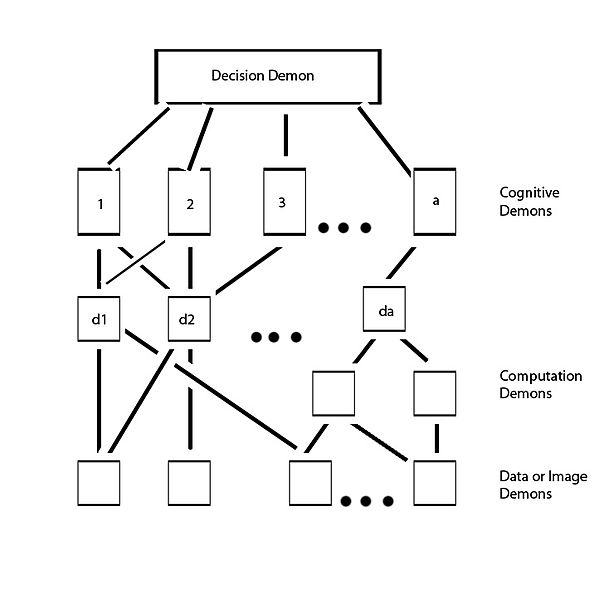
\includegraphics[scale=.65]{Images/Original_pande2.jpg}
\caption{The concept of pandemonium architecture }
\end{figure}
This approach although pioneering but suffered several criticisms , for example it was argued that it needs a large number of training examples to be able to catch the different possible patterns which may lead to it suffering from the same template matching problems \cite{minsky69perceptrons}, also most of the researches done building on the  pandemonium architecture are towards a restricted area of recognition of simple hand drawings like written 
letters and generalizing those results to other areas of recognition may be misleading \cite{Grainger2008}. 

Years after that another Hubel and Wiesel inspired attempt have been made by Fukushima in the early 1980s \cite{FukushimaM82} \cite{Fukushima1988}, Neocognitron is a multilevel neural network can be used for visual pattern recognition. Figure 2 shows the neocognitro architecture where is the lowest layer is used as an input layer. Each cell in a layer receives input from the layer directly before it's layer by being connected to the cells in a restricted area of this layer called it's  receptive fields.The layers in this structure is divided in two groups based on the cell type of each layer. Those layers are alternatively organized so that each "C-Cells" layer is succeeded by an "S-Cells" layers plus the first layer which is the input layer and the last layer which is a "C-Cells" recognition layer.

\begin{figure}[hbtp]
\centering
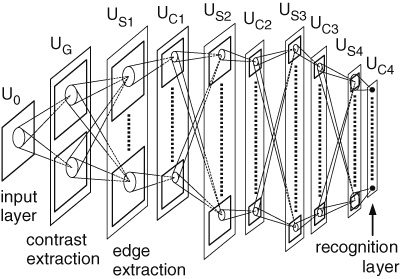
\includegraphics[scale=1]{Images/ScholarFig1.jpg}
\caption{A typical neocognitron architecture (courtesy of Kunihiko Fukushima) }
\end{figure}
\textbf{S-Cells} works as features extractors , their input connections are variable and is changed by the learning process. The learning process determine the selective response of each s-cell towards the particular features present in it's receptive field.While \textbf{C-Cells} are fixed invariable cells that receive it's input from s-cells , each c-cell receive it's input from a group of s-cells that are trained to extract the same feature from different places in the image and give an output signal if at least one s-cell in it's receptive field  gives an excitatory output so that if an feature changed it's position and the s-cell that responds is changed the c-cell will continue giving the same output.

During the training process the lower C-Cells extract the local features and the S-Cells tolerate the change in position of this features and gradually this local features build up into global features, and since s-cells tolerate some of the errors from the lower c-levels, s-cells at the highest levels gives robust responses to specific features even if it's slightly deformed. At the highest level C-cell works as recognition layer as it's integrate the information from all the previous levels, each cell responds only to one specific pattern even if the pattern is deformed , shifted in position , or changed in size. neocognitron is found in  many different application like optical character recognition and it's advances and ingenuity is the base for many other advances in the area of deep learning.

At the middle of the 1980s the Boltzmann Machine has been invented  by Hinton \& Sejnowski \cite{HintonSejnowski83} \cite{Hinton1986} a stochastic neural network type that is composed of symmetrically connected units and is capable of learning internal features from the data. Typically a Boltzmann machine can be used in search and learning problems but we are here will be focusing on the learning problem. The Boltzmann machine can be trained by several data vectors and it can then it can generate those data vectors. There are two general structures of the Boltzmann machine one that have only visible units and the other can have hidden units also.The Boltzmann Machine had a major problem that prevented using it in a large scale application, as the number of neurons increase the learning time increase rapidly and the 
learning become very slow. In 1986 Smolensky invented the Restricted Boltzmann Machine \cite{Smolensky86} it consists as the normal Boltzmann Machine with the restriction that its neurons form a Bipartite graph and it have only connection between the hidden units and the visible units and no connections are between units from the same layer. The learning of the RBMs require taking several iterations using the training data and re-adjusting the connections weights using different learning rules. As we will see below RBMs can be used in deep learning by constructing multiple RMBs one over the other and using the results from one machine as the data for the next one.

Nowadays deep learning is getting more and more of the interest from computer science researchers and a lot of effort have been given toward solving different problems in different research areas using deep learning algorithms like speech recognition , signal processing, natural language processing and object recognition. 

In 2006 Hinton \cite{Hinton2006D} introduced the generative deep belief networks that uses RBMs as it's basis , the Deep belief network can be viewed as a set of RBMs stacked one over the other and each layer receives it's connection from the output units of the RBMs in the previous layer and it's learning algorithm learn layer by layer. The first layer uses the training data and the learning rule and algorithm and backpropagating the error to adjust it's it's weights to achieve better performance, and then the output of this layer is used as input for the next layer and so on. Hinton reported \cite{Hinton2006D} the results of using the deep belief network for classifying the MNIST dataset. The whole training time of the network was about one week , and the error rate of the best model was 1.25\%. This method while introduced a new way of training neural networks suffered from some limitations (some of them was solved and will be mentioned in the next section) it works well with binary images but for a nonbinary values in images it's treated as probabilities, it's not translation invariant \cite{Lee2009} and scaling the algorithm up to work with real size images was a challenge at this time. 

In he same year Hinton \cite{HintonSalakhutdinov2006b} showed how a high-dimensional data can be reduced to lower dimensions data using pre-trained autoencoders, and showed that this yields a better results than the most common method Principal Component Analysis (PCA).The idea behind this research was using two sets of neural networks (encoder \& decoder) one to produce lower dimensional data from the input and the other can reconstruct the original data from the lower dimensional results (see figure 3). Using several layers of RBMs stacked over each other the decoder and the encoder were built.The learning process begins with pretraining where each RBMs is learned alone and the activated feature resulting from each layer are presented to the next layer as the input the layers  after then are unrolled together to create the autoencoder. After that comer the global fine tuning stage where backpropagation is used through the whole system to fine-tune the weights for optimal reconstruction. The system was tested against the sate-of-art algorithms PCA and latent semantic analysis (LSA) it was showen that the autoencoders gave much better reconstruction of the original data than both of those algorithms  the tasks where among image reduction and reconstruction from the MNIST dataset and Olivetti face dataset and in both the Autoencoders gave better performance and the usage of pretraining stage gave better performance than without using it.
\ref{Hinton2006D}
\begin{figure}[hbtp]
\caption{Autoencoders used in diminsionality reduction (Courtesy of George Hinton)}
\centering
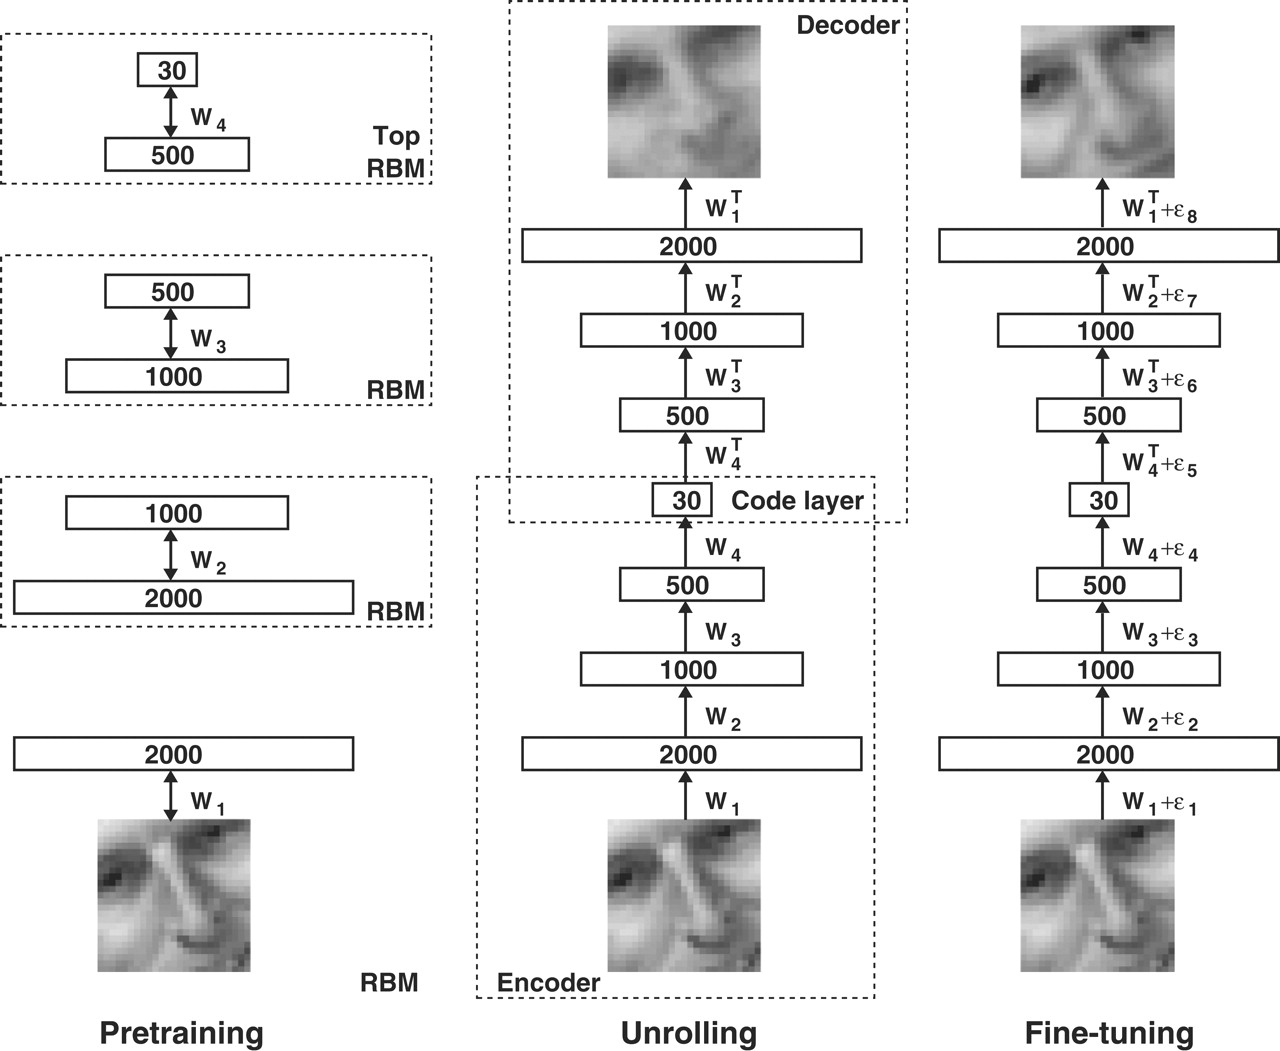
\includegraphics[scale=.30]{Images/autoencoders.jpg}
\end{figure}



\section{Deep Learning for detection and classification}
\label{sec:DLDC}
\subsection{Convolutional Deep Belief Networks}
This paper \cite{Lee2009} builds upon the previously introduced concept of the deep belief networks building a generative model of images with unsupervised learning.This paper addresses some of he issues mentioned before and other issues in dealing with larger images and make the model translation invariant to deal with having the objects in different places in image.The model have feature detectors that learns features in different location in the image, because feature detector that is able to learn information from one part of the image can be used to learn the same info from other parts though building a model that can learn large images using relatively small number of detectors.

This paper uses Convolution RBM rather than normal RBM the difference is that the CRBM share the weights of the hidden and visible layers are shared between all the locations in the image.
the CRBM consists of two layers Visible layer \textit{V} and hidden layer \textit{H}. The visible layer contains $ N \times N $ binary input units, while the hidden unit contains \textit{K} groups of units, each group contains $ M \times M $ binary units ( a total of $ M^2 \times K$ units) and each of those \textit{K} groups is associated with a $ J \times J $ filter , this filter weights are shared with all the units in the hidden group. Plus each hidden group $ K _{i} $ has a bias $ b _{k} $  and all the visible layer units have a shared bias \textit{c}.A layer of probabilistic max-pooling is then added as the final layer to allow for covering larger areas of the input in the higher layers in a probabilistically sound way see Figure 4.

\begin{figure}[hbtp]
\centering
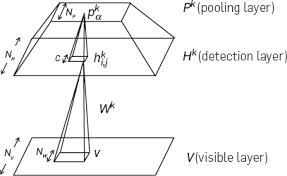
\includegraphics[scale=1]{Images/images.jpg}
\caption{max-pooling CRBM (Coutresy of Honglak Lee)}
\end{figure}

The max pooling layer is intended to " layers, which shrink the representation of the detection layers by a constant factor." \cite{Lee2009} which is computing the maximum activation of a small group of units in the detection layer (Hidden layer) this enables toleration the change in the features places and allow for the CRBM to be translation invariant. max pooling also helps speeding up the algorithm it was found  that the algorithm is 10 times slower without the 
max pooling layer.

The CRBM model is overcomplete that the size of the input is much smaller than the network representation of it since there are \textit{K} hidden groups each roughly of the size of an image, This may lead to the problem of overcomplete models which have the risk of detecting trivial features of the image and having a feature detector that represent single pixel of the input. While a common approach is to force sparse representation where a tiny fraction of the units are active given a specific stimulus, In this paper regularization was used to make the mean activation for each unit close some small constant.

The final network consists of several max-pooling CRBMs stacked one over the other and the final network energy function that is the sum of the energy functions for all of the individual layers. The training for this network is using the same greedy methods described in section 2 \cite{HintonSalakhutdinov2006b}.

\subsection{Experimental results for Classification and recognition}
To prove the validity of the approach the research team experimented the model against the state-of-art algorithms in well known tasks.The results then reported compared to the other algorithms.

At first the team approached  the Caltech-101 object classification task. The model was two layers of CRBMs the first layer was 24 groups of $10 \times 10$ pixels each, and the second layer was 100 groups of $10 \times 10$ pixels each. The CDBN gave test accuracy of $57.7 \pm 1.5\%$ when trained with 15 image per class and gave $65.4 \pm 0.5\%$ when trained with 30 image per class,while the Scale-invariant feature transform (SIFT) gave test accuracy of $54.0 \%$ when trained with 15 image per class and gave $64.6 \%$ when trained with 30 image per class, and shape-context gave  $59.0 \pm 0.56\%$ with 15 image and $66.2 \pm 0.5\%$ with 30.
It worth mentioning that the training for he CDBN was from natural scenes which are not related to the task and this means that CDBN acquired a general representation of the images that enabled it to recognize objects in new images with reasonable success rate compared to the state-of-art algorithms.

The CDBN was also used for classifying the MNIST dataset with a model of two layers  the first layer was 40 groups of $12 \times 12$ pixels each, and the second layer was 40 groups of $6 \times 6$ pixels each, this structure allowed the learning of digits characteristics in the two layers where the first layer learned the strokes of the digits and the second layer combined those strokes and learned the bigger parts of the digits. A feature vector was then constructed from those features and using a SVM those features were classified. This method made it possible to achieve 0.82\% test error which is much more the reported results of 1.2\% by Hinton and Salakhutdinov descried in section 2.

Then a 3 layers CDBN was trained on unlabeled images randomly selected from four different object categories (cars, faces, motorbikes, and airplanes) and the results of the classification in the form of \textit{AUC-PR} is reported per layer to show the ability of the CDBN to combine the features layer by layer to allow for better performance see [Table 1].\\

\begin{tabular}{|l c c r|}
\hline
    Layer & Faces & Motorbikes & Cars \\
\hline
First & $0.39 \pm 0.17$ & $0.44\pm0.21$  & $0.43\pm0.19$ \\
Second  & $0.86\pm0.13$ & $0.69\pm0.22$ &  $0.72\pm0.23$ \\
Third & $0.95\pm0.03$ & $0.81\pm0.13$ &  $0.87\pm0.15$ \\
\hline   
\end{tabular}
\captionof{table}{Average AUC-PR for each classification class per layer\\}


Those results shows that the Convolution deep believe network has the ability to learn underlying statistics of the input data in several levels and have a promising performance compared to the state-of-art algorithms in different AI tasks it was exploited to.

\section{Conclusion}
\label{sec:concl}
Deep learning architecture us a multilevel feature detectors where lower levels detect simple features and the higher levels detect more complex global features. There have been a lot of interest and development in the area of deep learning and it's ability to learn without a supervisor makes it reasonable to use with inf several applications that have a great amount of data and will be impractical to label all of this data.There are an increasing number of new research in the deep learning area, new algorithms are being developed for different applications. Finally deep learning is a promising learning field and can be used and gives results that are comparable to the state-of-art algorithms in most of the cases it was used in.

%%%%%%%%%%%%%%%%%%%%%%%%%%%%%%%%%%%%%%
% hier werden - zum Ende des Textes - die bibliographischen Referenzen
% eingebunden
%
% Insbesondere stehen die eigentlichen Informationen in der Datei
% ``bib.bib''
%
\bibliography{bib}
\bibliographystyle{plain}
\addcontentsline{toc}{section}{Bibliography}% Add to the TOC

\end{document}


